\Variant{03.10.2026 (2-smena)}
\QQ{1}{$255255$ sonining neçta natural böluvçisi bor?
\Opts{$32$}{$64$}{$48$}{$128$}}
\QQ{2}{Quyidagilardan neçtasi haqiqiy son?
\[1)\ \sqrt[3]{2-\sqrt5};\qquad 2)\ \sqrt{-144};\qquad 3)\ -\sqrt{64};\qquad 4)\ \sqrt{\sqrt{157}-13};\qquad 5)\ 3{,}8(6)\]
\Opts{$2$ ta}{$3$ ta}{$5$ ta}{$4$ ta}}
\QQ{3}{Tulki va it orasidagi masofa $120$ m. Tulki minutiga $320$ m, it esa minutiga $350$ m tezlik bilan bir yönalişda yugurmoqda. Neça minutdan keyin it tulkiga yetib oladi?
\Opts{$4$}{$5$}{$6$}{$3$}}
\QQ{4}{10-A sinf öquvçilarining $12\%$ i testni bajarmadi, $32\%$ i notöğri bajardi, qolgan $14$ nafari esa töğri bajardi. Sinfda neçta öquvçi bor?
\Opts{$25$}{$28$}{$30$}{$20$}}
\QQ{5}{$n$ ning qanday eng kiçik natural qiymatida ifodaning qiymati natural son böladi?
\[\left(\frac12\right)^{26}\cdot\left(\frac14\right)^{12}\cdot\left(\frac18\right)^5\cdot2^n\]
\Opts{$36$}{$47$}{$74$}{$65$}}
\QQ{6}{Hisoblang:
\[\sqrt[3]{9+4\sqrt5}+\sqrt[3]{9-4\sqrt5}\]
\Opts{$-\sqrt5$}{$\sqrt5$}{$3$}{$2\sqrt5$}}
\QQ{7}{$n$ ning qanday eng kiçik natural qiymatida $\sqrt{100+\sqrt n}+\sqrt{100-\sqrt n}$ ifodaning qiymati natural son böladi?
\Opts{$6156$}{$5184$}{$9216$}{$7200$}}
\QQ{8}{Arifmetik progressiyada $a_2+a_{10}=20$ va $a_1\cdot a_2=10$. $a_3$ ni toping.
\Opts{$1$}{$\dfrac{11}2$}{$1$ yoki $\dfrac{11}2$}{$-2$ yoki $4$}}
\QQ{9}{$(a_n)$ — arifmetik progressiya, $(b_n)$ — geometrik progressiya. Agar $a_1=b_1$, $a_2=b_2$ va $a_7=b_3$ bölsa, geometrik progressiyaning maxrajini toping.
\Opts{$3$}{$6$}{$4$}{$5$}}
\QQ{10}{Ifodani soddalaştiring:
\[\frac{\left(x^2-\dfrac1{y^2}\right)^x\left(y+\dfrac1x\right)^{y-x}}{\left(y^2-\dfrac1{x^2}\right)^y\left(x-\dfrac1y\right)^{x-y}}\]
\Opts{$\left(\dfrac yx\right)^{x+y}$}{$\left(\dfrac xy\right)^{x-y}$}{$\left(\dfrac xy\right)^{x+y}$}{$\left(\dfrac yx\right)^{x-y}$}}
\QQ{11}{$x+y\ne z$ bölsa, ifodani soddalaştiring:
\[\frac{x+y+z}{(x+y)^2-z^2}\cdot\left(x^2-y^2-z^2+2yz\right)\]
\Opts{$x-y+z$}{$x+y+z$}{$x+y-z$}{$(x+y+z)(x-y+z)$}}
\QQ{12}{Hisoblang:
\[\left(\sqrt[3]7\right)^{\frac3{\log_27}}-\log_49\cdot\log_913\cdot\log_{13}6+\log_424\]
\Opts{$1$}{$2$}{$3$}{$0$}}
\QQ{13}{Hisoblang:
\[\left(\frac1{\sin^240^\circ}-\frac1{\cos^240^\circ}\right)\cdot\frac{2\sin80^\circ\cdot\tg40^\circ}{1-\tg^240^\circ}\]
\Opts{$4$}{$2$}{$1$}{$8$}}
\QQ{14}{Hisoblang:
\[\frac1{\sin\frac\pi{14}}-4\cos\frac{2\pi}7\]
\Opts{$1$}{$2$}{$4$}{$\dfrac12$}}
\QQ{15}{Tenglama neçta haqiqiy ildizga ega?
\[15^x-2\cdot5^{x+2}+300=2\cdot3^{x+1}\]
\Opts{$1$ ta}{$2$ ta}{$3$ ta}{haqiqiy yeçimga ega emas}}
\QQ{16}{Tengsizlikni qanoatlantiruvçi butun sonlar neçta?
\[\sqrt{x-2}-\sqrt[4]{6-x}\ge0\]
\Opts{$4$}{$2$}{$3$}{$5$}}
\QQ{17}{Tengsizlikning butun yeçimlari yiğindisini toping:
\[\frac{8x+43}{\left(x^2+11x+24\right)(x+6)^2}-\frac1{x^2+9x+18}\ge0\]
\Opts{$-21$}{$-9$}{$-15$}{$-8$}}
\QQ{18}{$\bigl||x-1|-2\bigr|=2$ tenglama neçta ildizga ega?
\Opts{$2$}{$4$}{$3$}{$1$}}
\QQ{19}{$a$ ning neçta butun qiymatida $x^2+12x+3a=0$ tenglama ikkita turli manfiy ildizga ega böladi?
\Opts{$10$}{$11$}{$12$}{$9$}}
\QQ{20}{$f(x)=2x-3$ bölsa, $3\bigl(f(2x)-2f(x-1)\bigr)$ ni toping.
\Opts{$7$}{$21$}{$12x-27$}{$-21$}}
\QQ{21}{$y=(ax)^2-12x+9$ funksiyaning nollari özaro teng bölsa, $a$ ning barça haqiqiy qiymatlari yiğindisini toping.
\Opts{$-4$}{$4$}{$0$}{$-2$}}
\QQ{22}{$f(x)=\left(x^2-2\right)^2+\left(x^3-2\right)^3$ bölsa, $f'(1)$ ni toping.
\Opts{$-5$}{$13$}{$9$}{$5$}}
\QQ{23}{Integralni hisoblang:
\[\int\limits_0^{13}\frac{x+1}{\sqrt[3]{2x+1}}\,dx\]
\Opts{$28$}{$33{,}3$}{$36{,}3$}{$39{,}3$}}
\QQ{24}{$A$, $B$ va $C$ nuqtalar markazi $O$ bölgan aylanada yotadi. $\angle OAB=15^\circ$ va $\angle OCB=10^\circ$ bölsa, $\beta=\angle AOC$ markaziy burçakni toping.
\qfig{\begin{tikzpicture}[scale=1.1,font=\small]
\coordinate (O) at (0,0); \coordinate (B) at (100:1.6); \coordinate (A) at (215:1.6); \coordinate (C) at (-35:1.6);
\draw (O) circle (1.6); \draw (A)--(B)--(C); \draw (A)--(O)--(C); \fill (O) circle (1.3pt);
\draw ($(O)+(215:0.3)$) arc[start angle=215,end angle=325,radius=0.3]; \node at (270:0.5) {$\beta$};
\node[above] at (B) {$B$}; \node[below left] at (A) {$A$}; \node[below right] at (C) {$C$}; \node[above] at (0,0.05) {$O$};
\end{tikzpicture}}
\Opts{$40^\circ$}{$30^\circ$}{$60^\circ$}{$50^\circ$}}
\QQ{25}{$ABCD$ kvadrat berilgan. Töğri çiziq $AD$ va $BC$ tomonlarni mos ravişda $L$ va $K$ nuqtalarda, $DC$ va $AB$ tomonlarning davomlarini esa $P$ va $E$ nuqtalarda kesadi. $PL=2$, $LK=5$ va $KE=3$ bölsa, kvadrat yuzini toping.
\qfig{\begin{tikzpicture}[scale=0.55,font=\small]
\coordinate (D) at (0,0); \coordinate (C) at (4.472,0); \coordinate (B) at (4.472,4.472); \coordinate (A) at (0,4.472);
\coordinate (P) at (-1.789,0); \coordinate (L) at (0,0.894); \coordinate (K) at (4.472,3.130); \coordinate (E) at (7.155,4.472);
\draw (A)--(B)--(C)--(D)--cycle; \draw (P)--(D); \draw (B)--(E); \draw (P)--(E);
\foreach \p in {P,L,K,E} \fill (\p) circle (1.5pt);
\node[above left] at (A) {$A$}; \node[above] at (B) {$B$}; \node[below right] at (C) {$C$}; \node[below] at (D) {$D$};
\node[below] at (P) {$P$}; \node[left] at (L) {$L$}; \node[right] at (K) {$K$}; \node[above] at (E) {$E$};
\node[above left] at ($(P)!0.5!(L)$) {$2$}; \node[above left] at ($(L)!0.5!(K)$) {$5$}; \node[below right] at ($(K)!0.5!(E)$) {$3$};
\end{tikzpicture}}
\Opts{$20$}{$25$}{$27$}{$24$}}
\QQ{26}{Teng yonli töğri burçakli uçburçakning katetlari $4\sqrt2$ ga teng. Uçburçak içidagi $E$ nuqtadan katetlargaça bölgan masofalar $x$ ga, gipotenuzagaça bölgan masofa esa $1$ ga teng. $x$ ni toping.
\qfig{\begin{tikzpicture}[scale=0.6,font=\small]
\coordinate (B) at (0,0); \coordinate (A) at (0,5.657); \coordinate (C) at (5.657,0); \coordinate (E) at (2.121,2.121);
\coordinate (N) at (0,2.121); \coordinate (K) at (2.121,0); \coordinate (P) at (2.828,2.828);
\draw (A)--(B)--(C)--cycle; \draw (N)--(E)--(K); \draw (E)--(P); \fill (E) circle (1.5pt);
\draw (0,0.3)--(0.3,0.3)--(0.3,0); \draw (0,2.421)--(0.3,2.421)--(0.3,2.121); \draw (2.121,0.3)--(2.421,0.3)--(2.421,0);
\draw ($(P)!0.3cm!(E)$)--($(P)!0.3cm!(E)+(P)!0.3cm!(C)-(P)$)--($(P)!0.3cm!(C)$);
\node[above] at ($(N)!0.5!(E)$) {$x$}; \node[right] at ($(K)!0.5!(E)$) {$x$}; \node[above left] at ($(E)!0.5!(P)$) {$1$};
\node[left] at (A) {$A$}; \node[below left] at (B) {$B$}; \node[below] at (C) {$C$}; \node[below left] at (E) {$E$};
\node[left] at (0,2.83) {$4\sqrt2$}; \node[below] at (3.9,0) {$4\sqrt2$};
\end{tikzpicture}}
\Opts{$3\sqrt2$}{$2\sqrt2$}{$1{,}5\sqrt2$}{$4{,}5\sqrt2$}}
\QQ{27}{$ABC$ uçburçakda $\angle CAB=60^\circ$, $AB=6$ va $BC=14$. $BL$ — bissektrisa, $BM$ — mediana. $BLM$ uçburçakning yuzini toping.
\qfig{\begin{tikzpicture}[scale=0.45,font=\small]
\coordinate (A) at (0,0); \coordinate (C) at (16,0); \coordinate (B) at (3,5.196); \coordinate (L) at (4.8,0); \coordinate (M) at (8,0);
\fill[qfill] (B)--(L)--(M)--cycle;
\draw (A)--(B)--(C)--cycle; \draw (B)--(L); \draw (B)--(M);
\draw ($(A)+(0:0.8)$) arc[start angle=0,end angle=60,radius=0.8]; \node at ($(A)+(30:1.3)$) {\scriptsize$60^\circ$};
\node[below left] at (A) {$A$}; \node[above] at (B) {$B$}; \node[below right] at (C) {$C$}; \node[below] at (L) {$L$}; \node[below] at (M) {$M$};
\node[left] at ($(A)!0.5!(B)$) {$6$}; \node[above right] at ($(B)!0.5!(C)$) {$14$};
\end{tikzpicture}}
\Opts{$\dfrac{24\sqrt3}5$}{$24\sqrt3$}{$12\sqrt3$}{$\dfrac{12\sqrt3}5$}}
\QQ{28}{$ABCDEFGH$ muntazam sakkizburçakning tomoni $4$ ga teng. $ACEG$ törtburçakning yuzini toping.
\qfig{\begin{tikzpicture}[scale=0.38,font=\small]
\foreach \n/\a in {A/112.5,B/67.5,C/22.5,D/-22.5,E/-67.5,F/-112.5,G/-157.5,H/157.5} {\coordinate (\n) at (\a:5.226); \node at (\a:5.95) {$\n$};}
\fill[qfill] (A)--(C)--(E)--(G)--cycle;
\draw (A)--(B)--(C)--(D)--(E)--(F)--(G)--(H)--cycle; \draw (A)--(C)--(E)--(G)--cycle;
\node[above] at (90:5.0) {$4$};
\end{tikzpicture}}
\Opts{$16+16\sqrt2$}{$32+16\sqrt2$}{$32+32\sqrt2$}{$64$}}
\QQ{29}{$\alpha$ va $\beta$ tekisliklar $l$ töğri çiziq böylab kesişadi va ular orasidagi ikki yoqli burçak $30^\circ$ ga teng. $\alpha$ tekislikda $ABC$ ($\angle C=90^\circ$) töğri burçakli uçburçak yotadi, uning $AC$ kateti $l$ töğri çiziqda joylaşgan. Agar $AC=2$ va $AB:AC=2$ bölsa, $B$ uçidan $\beta$ tekislikkaça bölgan masofa neçaga teng?
\Opts{$\sqrt3$}{$\dfrac{\sqrt3}2$}{$2\sqrt3$}{$2\sqrt2$}}
\QQ{30}{$\vec a=(2;\,m;\,1)$ va $\vec b=(n;\,3;\,2)$ vektorlar kollinear. $mn$ köpaytmaning qiymatini toping.
\Opts{$4$}{$3$}{$8$}{$6$}}
\QQ{31}{Agar $B\subset A$ bölsa, $A\cap B$ ni toping.
\Opts{$A$}{$B$}{$A\cup B$}{$\varnothing$}}
\QQ{32}{$\underbrace{\overline{abcabc\ldots abc}}_{2025\ \text{xonali}}$ körinişdagi $2025$ xonali sonlar neçta? (Bu yerda $a$, $b$, $c$ — turli raqamlar.)
\Opts{$1000$}{$900$}{$720$}{$648$}}
\QQ{33}{\Moslash{Muntazam oltiburçakli piramidaga şar içki çizilgan bölib, uning apofemasi va asos tekisligi orasidagi burçagi $60^\circ$ ga teng. (Bunda $\pi=3$ deb oling.)
\par\centering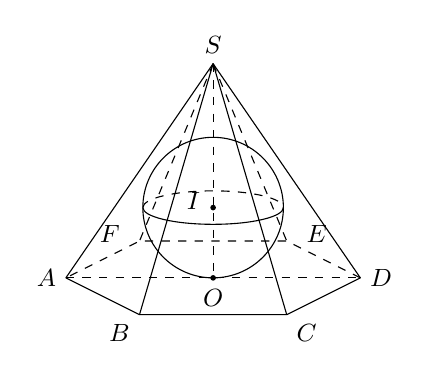
\begin{tikzpicture}[scale=0.85,font=\small]
\coordinate (A) at (-2.2,0); \coordinate (B) at (-1.1,-0.55); \coordinate (C) at (1.1,-0.55); \coordinate (D) at (2.2,0); \coordinate (E) at (1.1,0.55); \coordinate (F) at (-1.1,0.55); \coordinate (S) at (0,3.2); \coordinate (O) at (0,0); \coordinate (I) at (0,1.05);
\draw (A)--(B)--(C)--(D); \draw[dashed] (D)--(E)--(F)--(A);
\draw (S)--(A); \draw (S)--(B); \draw (S)--(C); \draw (S)--(D); \draw[dashed] (S)--(E); \draw[dashed] (S)--(F); \draw[dashed] (S)--(O); \draw[dashed] (A)--(D);
\draw (I) circle (1.05); \draw[dashed] (-1.05,1.05) arc (180:0:1.05 and 0.25); \draw (-1.05,1.05) arc (180:360:1.05 and 0.25);
\fill (I) circle (1.2pt); \fill (O) circle (1.2pt);
\node[above] at (S) {$S$}; \node[left] at (A) {$A$}; \node[below left] at (B) {$B$}; \node[below right] at (C) {$C$}; \node[right] at (D) {$D$}; \node[right] at (1.25,0.65) {$E$}; \node[left] at (-1.25,0.65) {$F$};
\node[below] at (0,-0.02) {$O$}; \node[left] at (-0.05,1.15) {$I$};
\end{tikzpicture}}{A) $\dfrac{\sqrt3}3$\par B) $\dfrac12$\par C) $\dfrac{2\sqrt3}9$\par D) $\dfrac13$\par E) $\dfrac{\sqrt3}2$\par F) $\dfrac29$}{Şar radiusining piramida balandligiga nisbatini toping.}{Şar sirtining piramida yon sirti yuziga nisbatini toping.}{Şar hajmining piramida hajmiga nisbatini toping.}}
\QQ{36}{Tenglamani yeçing:
\[\left(99+70\sqrt2\right)^x-7\left(17+12\sqrt2\right)^x+8\left(3+2\sqrt2\right)^x+\left(3-2\sqrt2\right)^x=7\]
\AB{Tenglama neçta haqiqiy ildizga ega?}{Tenglamaning haqiqiy ildizlari yiğindisini toping.}}
\QQ{37}{Tenglamani yeçing:
\[\frac{\sqrt3}2\,\tg\left(\frac{\pi-x}2\right)+\sin\left(\frac{3\pi}2-x\right)=1\]
\AB{Tenglamaning eng katta manfiy va eng kiçik musbat ildizlari yiğindisini toping.}{Tenglamaning $[0;\,\pi]$ oraliqdagi ildizlari sonini toping.}}
\QQ{38}{$f(x-1)=x+g(x)$ va $g(x-1)=x^2+1$ bölsa,
\AB{$f(2)$ ni toping.}{$f(x)=0$ tenglama neçta haqiqiy ildizga ega?}}
\QQ{39}{$P(x)=x^3+ax^2+bx+c$ köphadni $(x-2)(x-3)$ ga bölganda qoldiq $R(x)$, $(x-1)(x-4)$ ga bölganda esa qoldiq $2R(x)$ ga teng. Agar $P(0)=-40$ bölsa,
\AB{$\dfrac{P'(-1)}{P(6)}$ ning qiymatini toping.}{$y=P(x)$ funksiyaning $[2;\,4]$ oraliqdagi eng katta qiymatini toping.}}
\QQ{40}{$f(x)=x^2+1$ va $y=3-x^2$ funksiyalar berilgan.
\AB{Ularning grafiklari orasida hosil bölgan sohani $Ox$ öqi atrofida aylantirişdan hosil bölgan jism hajmini toping.}{Ularning grafiklari orasida hosil bölgan sohani $Oy$ öqi atrofida aylantirişdan hosil bölgan jism hajmini toping.}}
\QQ{41}{$ABC$ uçburçakda $BC=17$ sm, $D$ nuqta $AC$ tomonning örtasi va $DC=9$ sm. Uçburçakka içki çizilgan aylana $AB$ tomonga $K$ nuqtada urinadi, aylana markazi esa $DK$ kesmada yotadi.
\qfig{\begin{tikzpicture}[scale=0.42,font=\small]
\coordinate (A) at (0,0); \coordinate (C) at (18,0); \coordinate (B) at (1.667,4.714); \coordinate (D) at (9,0); \coordinate (K) at (1,2.828); \coordinate (I) at (3,2.121);
\draw (A)--(B)--(C)--cycle; \draw (I) circle (2.121); \draw (K)--(D); \fill (I) circle (2.5pt);
\draw (4.5,-0.2)--(4.5,0.2); \draw (4.6,-0.2)--(4.6,0.2); \draw (13.45,-0.2)--(13.45,0.2); \draw (13.55,-0.2)--(13.55,0.2);
\node[below left] at (A) {$A$}; \node[above] at (B) {$B$}; \node[below right] at (C) {$C$}; \node[below] at (D) {$D$}; \node[left] at (K) {$K$}; \node[above] at (3.1,2.2) {$I$};
\node[above right] at ($(B)!0.5!(C)$) {$17$}; \node[below] at (13.5,-0.2) {$9$};
\end{tikzpicture}}
\AB{$AB$ kesma uzunligini toping.}{Aylana radiusini toping.}}
\QQ{42}{Teng yonli $ABCD$ trapetsiyaning asoslari $BC=7$ va $AD=25$. Uning $AC$ diagonali $CD$ yon tomoniga perpendikulyar, $CH$ esa trapetsiya balandligi. $ABC$ uçburçakka aylana içki çizilgan.
\qfig{\begin{tikzpicture}[scale=0.26,font=\small]
\coordinate (A) at (0,0); \coordinate (D) at (25,0); \coordinate (B) at (9,12); \coordinate (C) at (16,12); \coordinate (H) at (16,0);
\draw (A)--(B)--(C)--(D)--cycle; \draw (A)--(C); \draw (C)--(H); \draw (10,10) circle (2);
\draw (16,0)--(15.2,0)--(15.2,0.8)--(16,0.8); \draw ($(C)!0.8cm!(A)$)--($(C)!0.8cm!(A)+(C)!0.8cm!(D)-(C)$)--($(C)!0.8cm!(D)$);
\node[below left] at (A) {$A$}; \node[above left] at (B) {$B$}; \node[above right] at (C) {$C$}; \node[below right] at (D) {$D$}; \node[below] at (H) {$H$};
\node[above] at (12.5,12) {$7$}; \node[below] at (8,0) {$25$};
\end{tikzpicture}}
\AB{Aylana radiusini toping.}{Trapetsiya yuzini toping.}}
\QQ{43}{Muntazam $ABCDEF$ oltiburçakning yuzi $6\sqrt3$ ga teng. $AD$ diagonal $BE$ va $CE$ diagonallarni mos ravişda $L$ va $K$ nuqtalarda, $DF$ diagonal esa $BE$ va $CE$ diagonallarni mos ravişda $M$ va $N$ nuqtalarda kesib ötadi.
\qfig{\begin{tikzpicture}[scale=1.15,font=\small]
\coordinate (B) at (-2,0); \coordinate (C) at (-1,1.732); \coordinate (D) at (1,1.732); \coordinate (E) at (2,0); \coordinate (F) at (1,-1.732); \coordinate (A) at (-1,-1.732);
\coordinate (L) at (0,0); \coordinate (K) at (0.5,0.866); \coordinate (M) at (1,0); \coordinate (N) at (1,0.577);
\fill[qfill2] (L)--(M)--(N)--(K)--cycle;
\draw (A)--(B)--(C)--(D)--(E)--(F)--cycle; \draw (A)--(D); \draw (B)--(E); \draw (C)--(E); \draw (D)--(F);
\node[below left] at (A) {$A$}; \node[left] at (B) {$B$}; \node[above left] at (C) {$C$}; \node[above right] at (D) {$D$}; \node[right] at (E) {$E$}; \node[below right] at (F) {$F$};
\node[above left] at (L) {$L$}; \node[above left] at (K) {$K$}; \node[below right] at (M) {$M$}; \node[above right] at (N) {$N$};
\end{tikzpicture}}
\AB{$LM$ kesma uzunligini toping.}{Böyalgan $LMNK$ soha yuzini toping.}}
\QQ{44}{Uçburçakli piramidaga şar içki çizilgan. Piramidaning yon qirralari özaro perpendikulyar va ularning uzunliklari $3$, $4$ va $7$ ga teng.
\AB{Piramidaning töla sirti yuzini toping.}{Içki çizilgan şar radiusini toping.}}
\QQ{45}{Qadahning yuqori qismi aylanma paraboloid şaklida bölib, uning yuqori asosining diametri $6$ sm, çuqurligi $9$ sm. Qadah içiga şar şaklidagi konfet tuşirildi. Konfet qadah devorlariga urinib turadi, konfetdan qadah tubigaça bölgan eng qisqa masofa $2{,}25$ sm.
\qfig{\begin{tikzpicture}[scale=0.36,font=\small]
\fill[qfill2] (0,6.25) circle (2); \draw (0,6.25) circle (2); \draw (-2,6.25) arc (180:360:2 and 0.4); \draw[dashed] (2,6.25) arc (0:180:2 and 0.4);
\draw[thick,domain=-3:3,samples=60] plot (\x,{\x*\x}); \draw[thick] (0,9) ellipse (3 and 0.5);
\draw (-0.35,0.12)--(-0.35,-8); \draw (0.35,0.12)--(0.35,-8); \draw (-0.35,-8) to[out=-90,in=0] (-3,-8.8); \draw (0.35,-8) to[out=-90,in=180] (3,-8.8);
\draw (0,-8.8) ellipse (3 and 0.45); \draw (-3,-8.8)--(-3,-9.2); \draw (3,-8.8)--(3,-9.2); \draw (-3,-9.2) arc (180:360:3 and 0.45);
\draw[{Stealth[length=3pt]}-{Stealth[length=3pt]}] (0,0)--(0,4.25); \node[right] at (0,2.4) {\tiny$2{,}25$};
\draw (-3,9.3)--(-3,10.6); \draw (3,9.3)--(3,10.6); \draw[{Stealth[length=3pt]}-{Stealth[length=3pt]}] (-3,10.3)--(3,10.3); \node[above] at (0,10.3) {$6$};
\draw (3.3,9)--(5.3,9); \draw (0.5,0)--(5.3,0); \draw[{Stealth[length=3pt]}-{Stealth[length=3pt]}] (5,0)--(5,9); \node[right] at (5,4.5) {$9$};
\end{tikzpicture}}
\AB{Qadahning hajmini toping.}{Konfetning hajmini toping.}}
\Javoblar{B B A A D C A C D C A C A B B C C C B B C D D D A C A B A D B D D A C}{\OK{36}{$2$}{$0$}\OK{37}{$-\dfrac{2\pi}3$}{$3$}\OK{38}{$20$}{$2$}\OK{39}{$4$}{$-4$}\OK{40}{$\dfrac{32\pi}3$}{$\pi$}\OK{41}{$5$}{$\dfrac{3\sqrt2}2$}\OK{42}{$2$}{$192$}\OK{43}{$1$}{$\dfrac{\sqrt3}3$}\OK{44}{$49$}{$\dfrac67$}\OK{45}{$\dfrac{81\pi}2$}{$\dfrac{32\pi}3$}}
